\chapter{State of the Art}
\label{chapter:sota}

In this chapter, we discuss the state of the Art on the topics of interest for this thesis, so as to provide an overview of recent developments in the field as well as to identify the open research problems and challenges in the area, some of which will be addressed in this thesis. 
The chapter starts describing some of the essential concepts as background information for the reader, about knowledge representation and annotation in the Web in \cref{sec:chp2_semweb}. 
Then, in \cref{sec:chp2_declarative_kgc}, we focus on describing current techniques to construct knowledge graphs, particularly with declarative approaches. 
The challenges in the adoption of declarative KGC approaches lead us to present the user-friendly approaches developed to facilitate the creation of the mapping documents in \cref{sec:chp2_easy_kgc}. Next, \cref{sec:chp2_kg_lifecycle} introduces several knowledge graph life cycle proposals, analysing in which stages declarative mappings can play a beneficial role for its management. 
The chapter concludes with \cref{sec:chp2_conclusions-sota} drawing the conclusions from each area of research and its main gaps, introducing how this thesis contributes to advance the state of the art. 


\section{Knowledge Representation in the Semantic Web}
\label{sec:chp2_semweb}

This section describes the concepts that play a relevant role in knowledge representation on the web, hence also relevant to its creation. First we present the Resource Description Framework (RDF)~\parencite{rdf}, used as backbone of knowledge graphs and also for specifying declarative transformation rules (\cref{sec:chp2_rdf}). Then, we discuss different approaches for annotating statements in RDF to add additional information (\cref{sec:chp2_reifications}).

\subsection{Resource Description Framework (RDF)}
\label{sec:chp2_rdf}

The Resource Description Framework (RDF)~\parencite{rdf} is a standard model for data interchange on the web. Its basic unit are triples: two concepts linked by a relationship. These triples are represented in the form of $<$ \textit{s,p,o} $>$, where \textit{s} is the subject, \textit{p} is the predicate and \textit{o} the object. This model relies on the use of the linking structure of the Web, using IRIs to identify uniquely every resource and relationship. 

\cref{lst:chp2_rdf-example} presents an example of an RDF graph composed of a set of triples about pole vault records, which is also visually depicted in \cref{fig:chp2_rdf-example}. In total there are four triples. They all share the same subject, which is a resource uniquely identified by the IRI $<$\texttt{http://example.com/athlete/1}$>$. Likewise, all predicates in the triples are also defined by an IRI, e.g. $<$\texttt{http://example.com/ns\#name}$>$. The first triple (Line 5) defines that the subject is an instance of the class \texttt{ex:Athlete} with the predicate \texttt{rdf:type}. The rest of the triples define attributes of this instance with name (\texttt{ex:name}) and position in the ranking (\texttt{ex:rank}). The objects of both triples are literals, that may be strings ("Yelena Isinbayeva", Line 6) or typed literals ("1"\scalebox{.8}{\textsuperscript{$\wedge\wedge$}}\texttt{xsd:integer}, Line 7). Type literals refer to data values attached with a tag that represents their data type.

\begin{minipage}{\textwidth}
\begin{captionedlisting}{lst:chp2_rdf-example}{Example of RDF graph.}
\centering
{\begin{lstlisting}[language=r2rml]
@prefix rdf: <http://www.w3.org/1999/02/22-rdf-syntax-ns#>.
@prefix xsd: <http://www.w3.org/2001/XMLSchema#>.
@prefix ex: <http://example.com/ns#>.

<http://example.com/athlete/1> rdf:type ex:Athlete .
<http://example.com/athlete/1> ex:name "Yelena Isinbayeva" .
<http://example.com/athlete/1> ex:rank "1"^^xsd:integer .
\end{lstlisting}}
\end{captionedlisting}
\end{minipage}

There are different syntaxes to serialize RDF graphs. RDF/XML\footnote{\url{https://www.w3.org/TR/rdf-syntax-grammar}} was the first to be proposed, and relies on XML. Notation3 (N3)\footnote{\url{https://www.w3.org/TeamSubmission/n3/}} was developed as a human readable syntax, but its use is not common. Instead, the N-Triples\footnote{\url{https://www.w3.org/TR/n-triples}} and Turtle\footnote{\url{https://www.w3.org/TR/turtle}} serializations, subsets of N3, are more widely used. JSON-LD\footnote{\url{https://www.w3.org/TR/json-ld11}} was developed for programming environments, as it is written in JSON documents. Lastly, RDFa\footnote{\url{https://www.w3.org/TR/rdfa-primer}} extends HTML to markup structured content in webpages, with the objective of improving the results retrieved by search engines. 



\begin{figure*}[t]
\centering
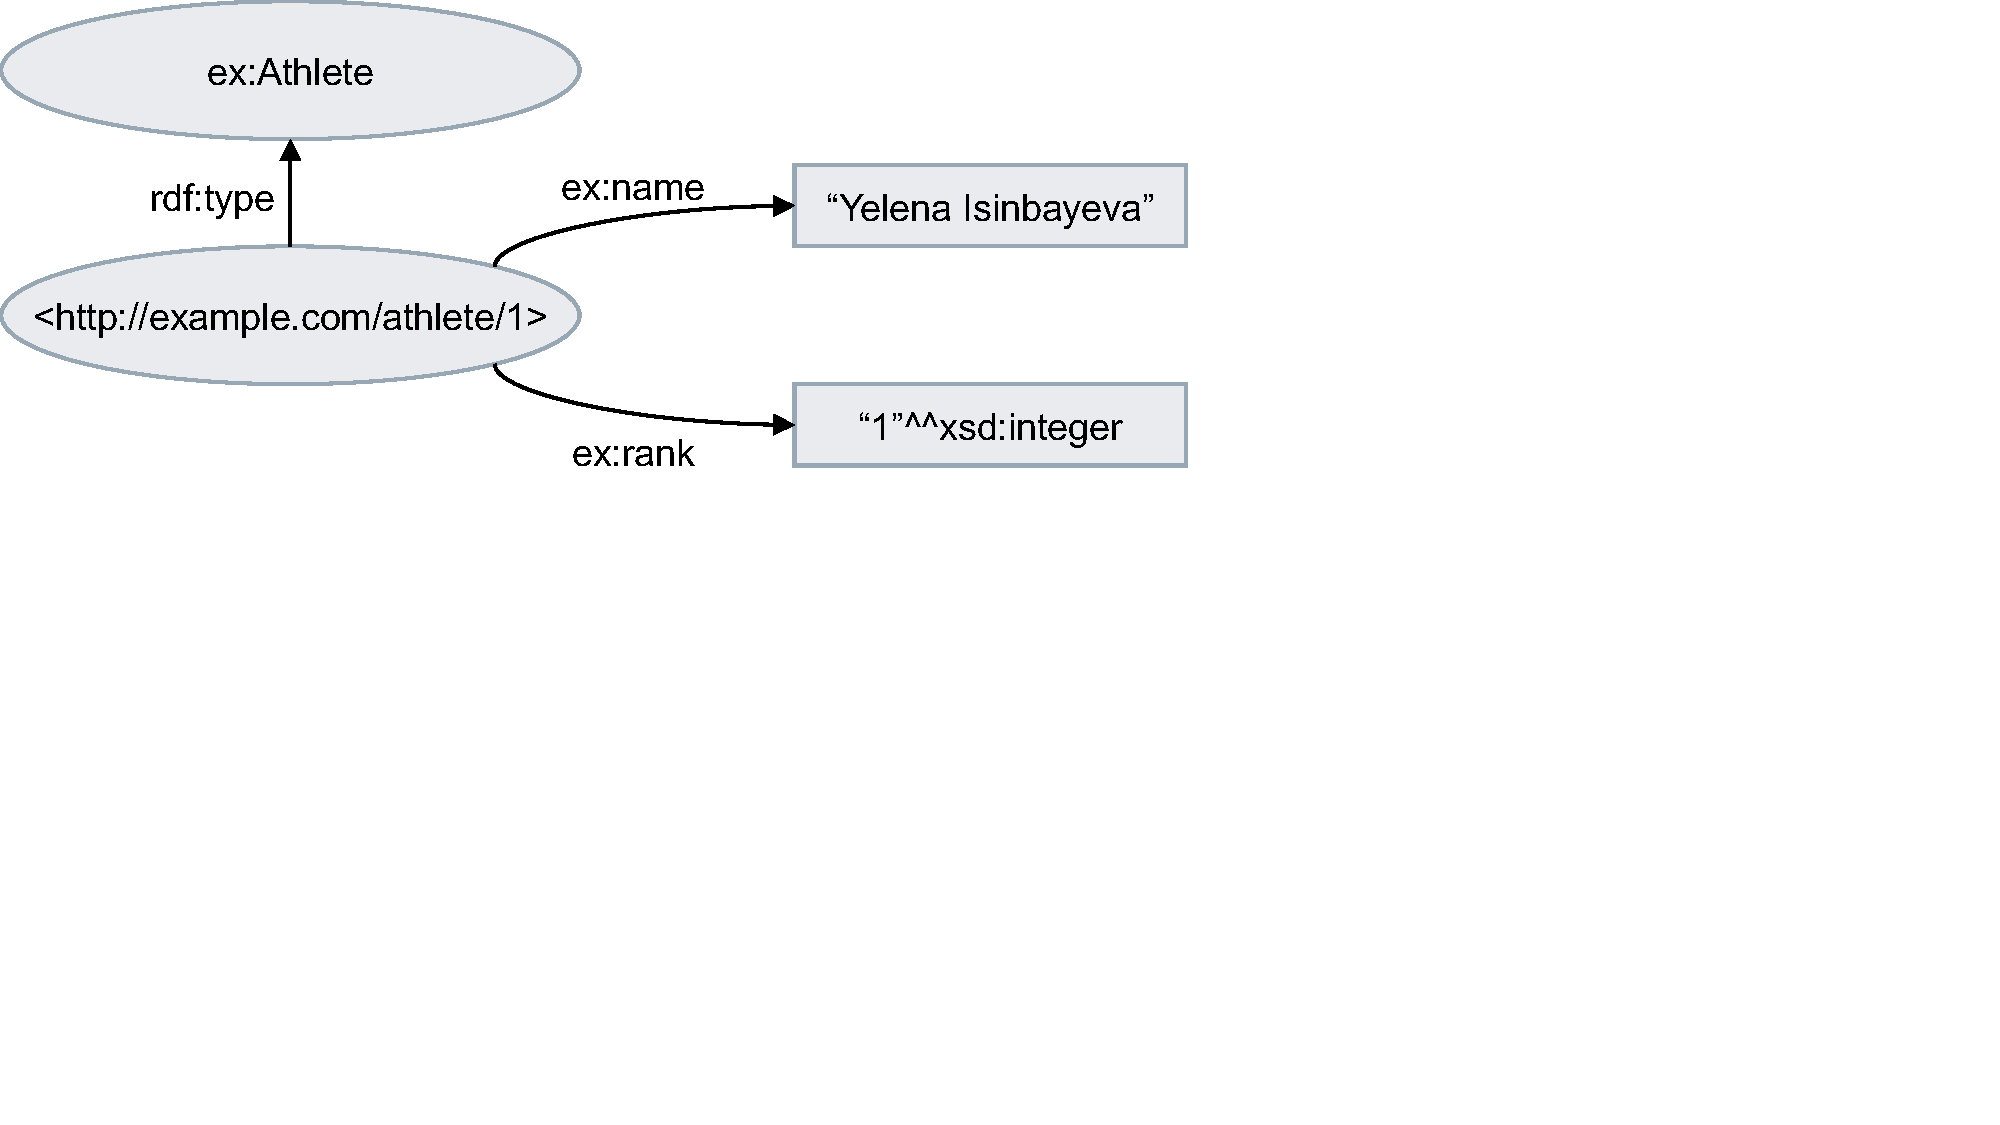
\includegraphics[width=0.6\linewidth]{figures/chp2_rdf-example.pdf}
\caption[RDF graph example]{Visual representation of the RDF graph shown in \cref{lst:chp2_rdf-example}.}
\label{fig:chp2_rdf-example}
\end{figure*}

\subsection{Statements about statements in RDF}
\label{sec:chp2_reifications}

%\ana{basic intro about what is this for and mot example about info that cannot be plainly represented in RDF. Then present all approaches used along the document: std reification, n-ary relationships, singleton properties, rdf-star, named graphs, i'd leave wikidata out of this}

Plain triples are not always able to represent the complexity of all knowledge. This is the case of statement annotation, when it is required to add information to a triple that does not correspond to a single resource, but the entire statement. This situation triggered the development different approaches to achieve triple annotation (or reification). \cref{fig:chp2_reification} illustrates instances of these models for the main statement \textit{Yelena Isinbayeva obtained the first position in the rank}, annotated with the additional statement \textit{in the season of 2009}. 

\begin{figure*}[t]
\centering
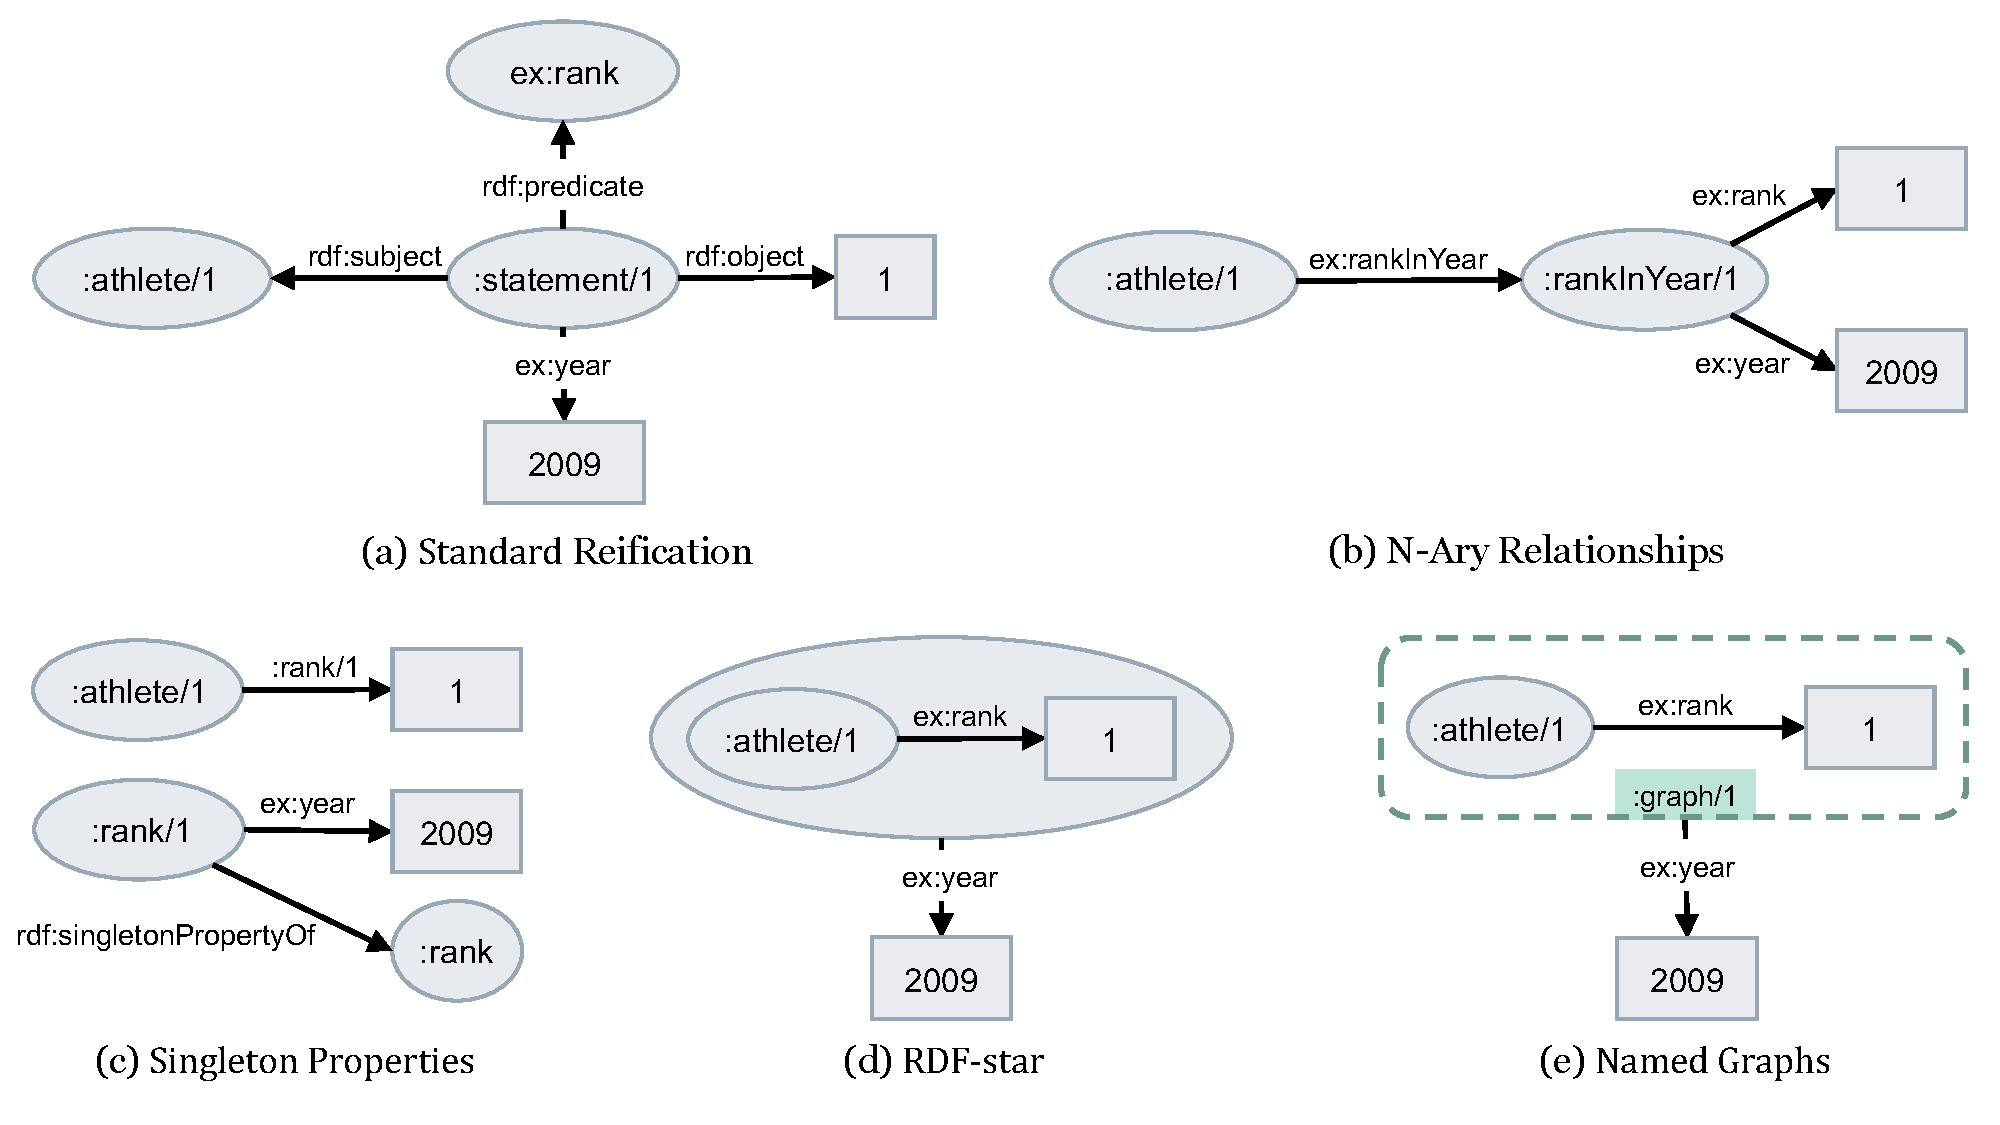
\includegraphics[width=\linewidth]{figures/chp2_reifications.pdf}
\caption[Approaches for statement reification in RDF]{Approaches for statement reification in RDF: (a) Standard Reification, (b) N-Ary Relationships, (c) Singleton Properties, (d) RDF-star and (e) Named Graphs.}
\label{fig:chp2_reification}
\end{figure*}

\noindent\textbf{Standard Reification}~\parencite{lassila1999rdf} explicitly declares a resource to denote an \texttt{rdf:Statement}.
This statement has \texttt{rdf:subject}, \texttt{rdf:predicate}, and \texttt{rdf:object} attached to it and can be further annotated with additional statements. The resource is typically a blank node, but an IRI can be used. 
In \cref{fig:chp2_reification}a, the resource \texttt{:statement/1} is an \texttt{rdf:Statement} with four associated triples, where the objects of the triples are the actual values of the triple (i.e. \texttt{:athlete/1} for the subject, \texttt{ex:rank} for the predicate, and \texttt{1} for the object). The property \texttt{ex:year} is used with its own value as object.


\noindent\textbf{N-Ary Relationships}~\parencite{naryw3c2006} converts a relationship into an instance that describes the relation, which can have attached both the main object and additional statements.
This representation is widely used in ontology engineering as an ontology design pattern~\parencite{gangemi2013multi}. In \cref{fig:chp2_reification}b, the entity \texttt{:athlete/1} points to an intermediate node (\texttt{:rankInYear/1}) which holds the triples for both the position in rank and year when it took place.

\noindent\textbf{Singleton Properties}~\parencite{nguyen2014don} uses unique predicates in the main triple. This unique predicate can then become the subject of the additional triple. The unique predicate is linked to the original predicate using \texttt{rdf:singletonPropertyOf}.
In \cref{fig:chp2_reification}c, the main triple uses the predicate \texttt{:rank/1}, the unique version of the original \texttt{ex:rank}. This predicate is then annotated with the year of the ranking. 

\noindent\textbf{RDF-star}~\parencite{hartig2017foundations,hartig2023rdf} extends RDF with a new syntax for compact triple reification. 
It introduces the notion of triple recursiveness with \texttt{Quoted Triples}, which can be used as subjects and/or objects of other triples. This is the only approach that extends the standard RDF features. 
%, having a potential impact on the development of supporting tools, triplestores, etc. 
This representation is currently being incorporated into the RDF 1.2 specification~\parencite{hartig2023rdf}, which is currently being developed under the RDF-star W3C Working Group\footnote{\url{https://www.w3.org/groups/wg/rdf-star/}}.
In Figure \ref{fig:chp2_reification}d we observe the example as an RDF-star graph, and it is represented in RDF as \texttt{{<<:athlete/1 ex:rank 1>> ex:year 2009}}.


\noindent\textbf{Named Graphs}~\parencite{rdf} are a SPARQL 1.1 feature that allows the assignment of an IRI to one or several triples as a graph identifier. Hence, graph IRIs allow the unique identification of triples. These IRIs can be used as subjects to add additional statements. 
In \cref{fig:chp2_reification}e, the main triple indicating the rank position of an athlete is assigned the named graph \texttt{:graph/1}. The graph IRI is subsequently used as subject in a triple that adds information about the year of the triple within the graph. 

\section{Knowledge Graph Construction with Declarative Mapping Rules}
\label{sec:chp2_declarative_kgc}

Knowledge graphs can be constructed in diverse manners. Some KGs are constructed natively in RDF by collecting knowledge from contributions of the community, such as Wikidata. Other KGs are constructed by transforming data from heterogeneous formats and sources, unstructured or (semi-)structured, into RDF. This section provides an overview of the latter, with a focus on declarative KG construction from heterogeneous data sources.

%\ana{overview de distintas formas y métodos en general de construir KGs. Debería ser algo larga, ampliando lo que hay en la intro. Luego terminar con enfocarse en los approaches declarativos, que se extienden en la siguiente subsección}

%\ana{RAW} In this section, the current scene of mapping languages is described first, regardless of the approach they follow, i.e., RDF materialization or virtualization. Then, previous works comparing mapping languages are surveyed. 


Constructing RDF knowledge graphs from heterogeneous data sources involves a schema transformation of the data to the desired graph structure. This transformation may be done in different ways, usually involving mapping languages that allow expressing the transformation rules to create the target graphs. Hence, these mappings hold declaratively the relationships between the source and target data schemas. This comprises an agnostic approach that can (and has been) applied to multiple different use cases, such as agriculture~\parencite{bilbao2022practical}, public procurement~\parencite{soylu2022theybuyforyou}, biomedicine~\parencite{iglesias2019bio2rdf,michel2020covid,aisopos2023knowledge}, cultural heritage~\parencite{calvanese2016culturalheritage}, IoT~\parencite{cimmino2020ewot,gonzalezgerpe2022extension}, among others.

The usual workflow in which declarative approaches are involved is depicted in \cref{fig:chp2_kgc-workflow}. They enable both materialization and virtualization of knowledge graphs. In materialization scenarios, data is transformed into the target graph, usually following the schema provided by an ontology. In virtualization scenarios, data is not transformed; instead, the original data source is accessed also following the schema of the target (virtual) graph. This process requires translating the original query into the language of the original data source. %\ana{mention OBDA?}

\begin{figure*}[h]
\centering
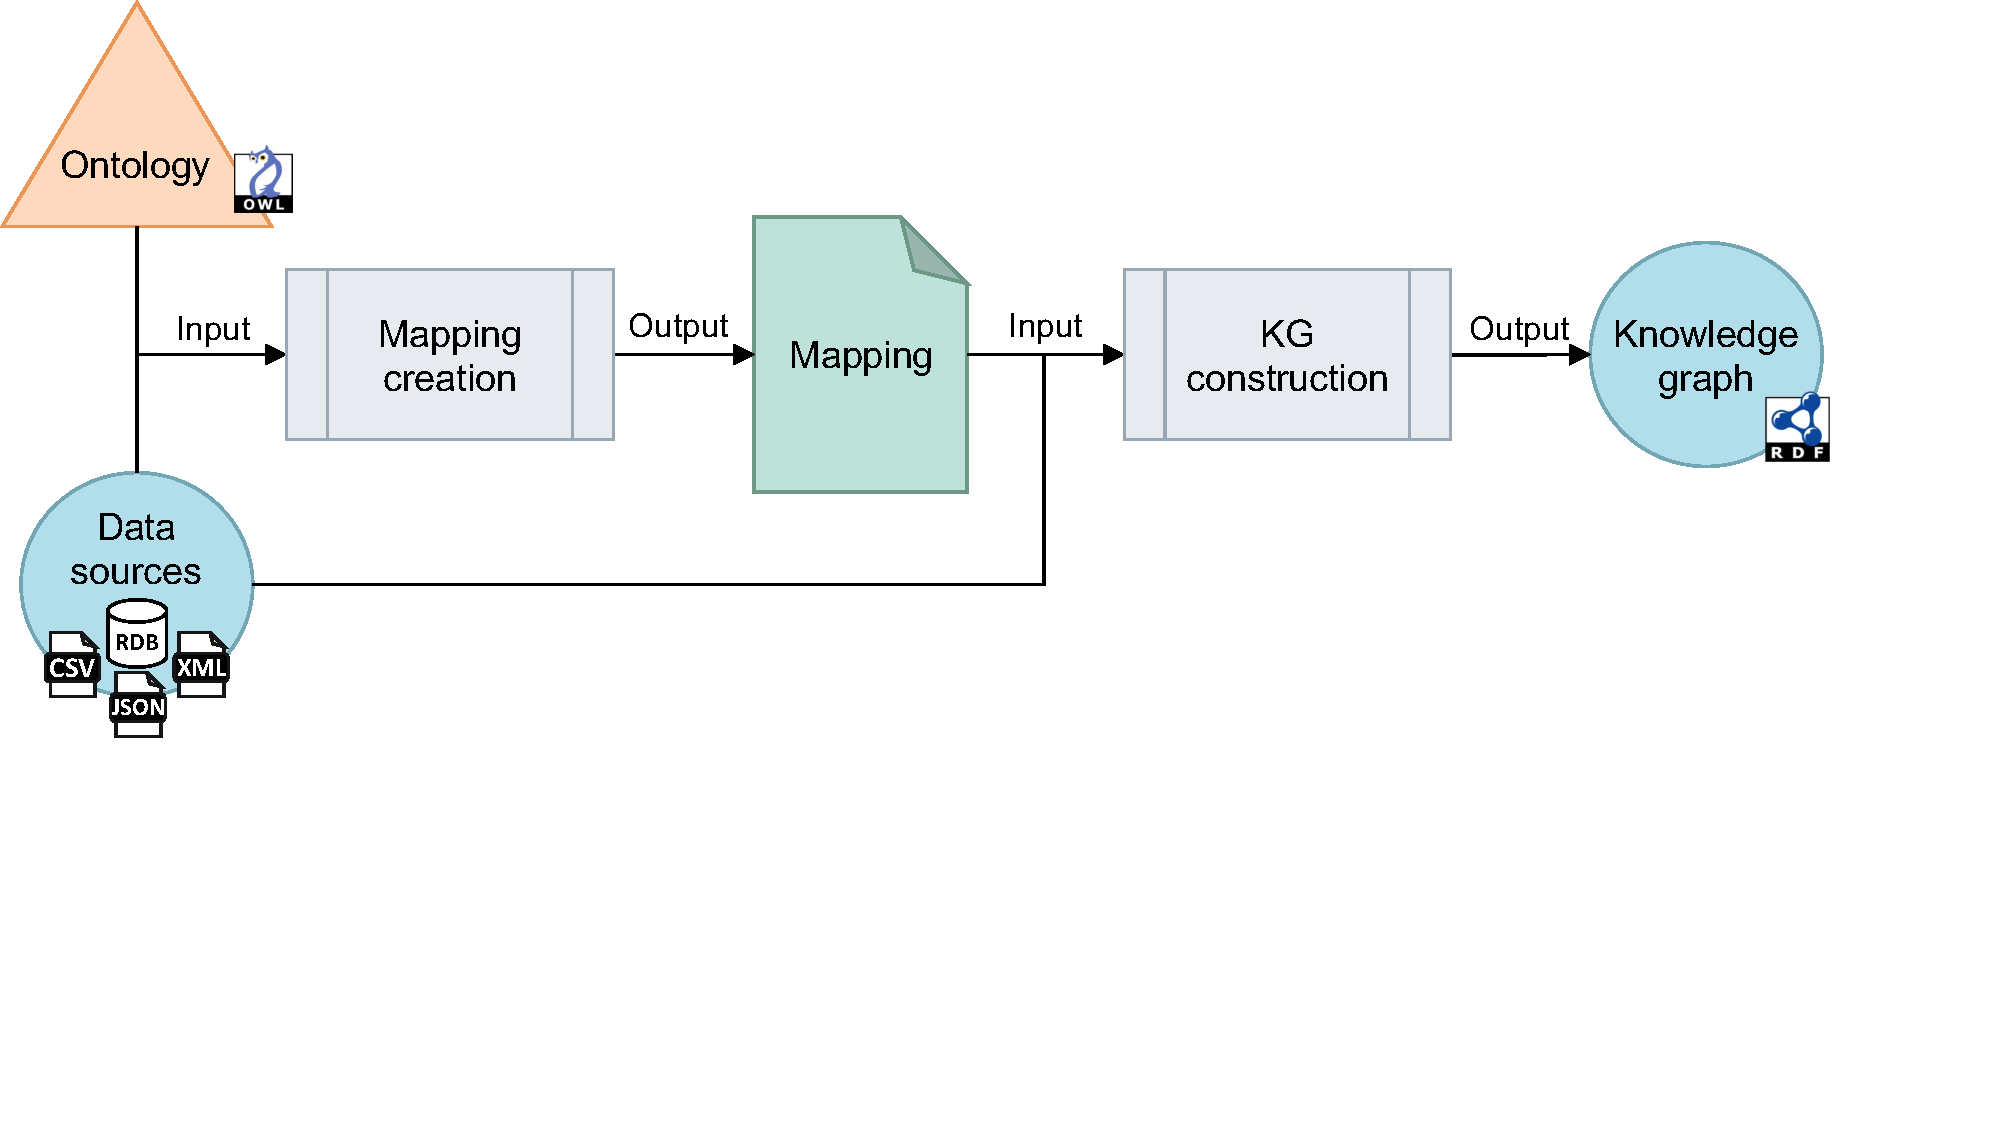
\includegraphics[width=0.9\linewidth]{figures/chp2_kgc-workflow.pdf}
\caption[Declarative knowledge graph construction workflow]{Declarative knowledge graph construction workflow.}
\label{fig:chp2_kgc-workflow}
\end{figure*}

This section presents an overview of existing mapping languages. We first show two well known RDF-based mapping languages that are widely adopted: the W3C Recommendation R2RML (\cref{sec:chp2_R2RML}), and its most relevant extension, RML (\cref{sec:chp2_RML}); and then other relevant languages (\cref{sec:chp2_more-languages}). Lastly, we discuss the approaches that compare the diversity and expressiveness of these mapping languages (\cref{sec:chp2_language-comparison}), and the current interoperability among them (\cref{sec:chp2_interoperability}).






\subsection{R2RML: RDB to RDF Mapping Language}
\label{sec:chp2_R2RML}

R2RML~\parencite{das2012r2rml} addresses the transformation of data in relational databases into RDF. This language specifies how to write the transformation rules in R2RML mapping documents. An R2RML mapping document is composed by at least one \textit{Triples Map} (\texttt{rr:TriplesMap}). \textit{Triples Maps} are used to define the transformation rules to generate RDF triples, their structure is depicted in \cref{fig:chp2_r2rml-tm}. It contains:

\begin{itemize}
    \item One \textit{Logical Table} (\texttt{rr:LogicalTable}), that describes the source relational table or view of a database.
    \item One \textit{Subject Map} (\texttt{rr:SubjectMap}), that defines how to generate the subject of the triples, and optionally, the corresponding class(es) it may be instance of (\texttt{rr:class}).
    \item Zero to multiple \textit{Predicate Object Maps} (\texttt{rr:PredicateObjectMap}). A \textit{Predicate Object Map} (POM) is formed by one to multiple \textit{Predicate Maps} (\texttt{rr:PredicateMap}), and one to many \textit{Object Maps} (\texttt{rr:ObjectMap}).% or \textit{Referencing Object Maps} (\texttt{rr:RefObjectMap}). The former is used for regular objects of triples, and the latter for creating as object the subject of another \textit{Triples Map}. 
\end{itemize}

\textit{Graph Maps} (\texttt{rr:GraphMap}) indicate how to generate named graphs. Zero or more \textit{Graph Maps} can be assigned to both \textit{Subject Maps} and \textit{Predicate Object Maps}. 
It is also possible to join \textit{Logical Tables} by replacing an \textit{Object Map} for a\textit{Referencing Object Map} (\texttt{rr:RefObjectMap}), which uses the subject of another \textit{Triples Map}, indicated with \texttt{rr:parentTriplesMap}, as the object of the triple. 
This join may have a condition to be performed, which is indicated using \texttt{rr:joinCondition}, \texttt{rr:child}, and \texttt{rr:parent}. 
Additionally, \textit{Object Maps} may include additional information, such as datatypes (\texttt{rr:datatype}) and languages (\texttt{rr:language}) of literals. 

\begin{figure*}[h]
\centering
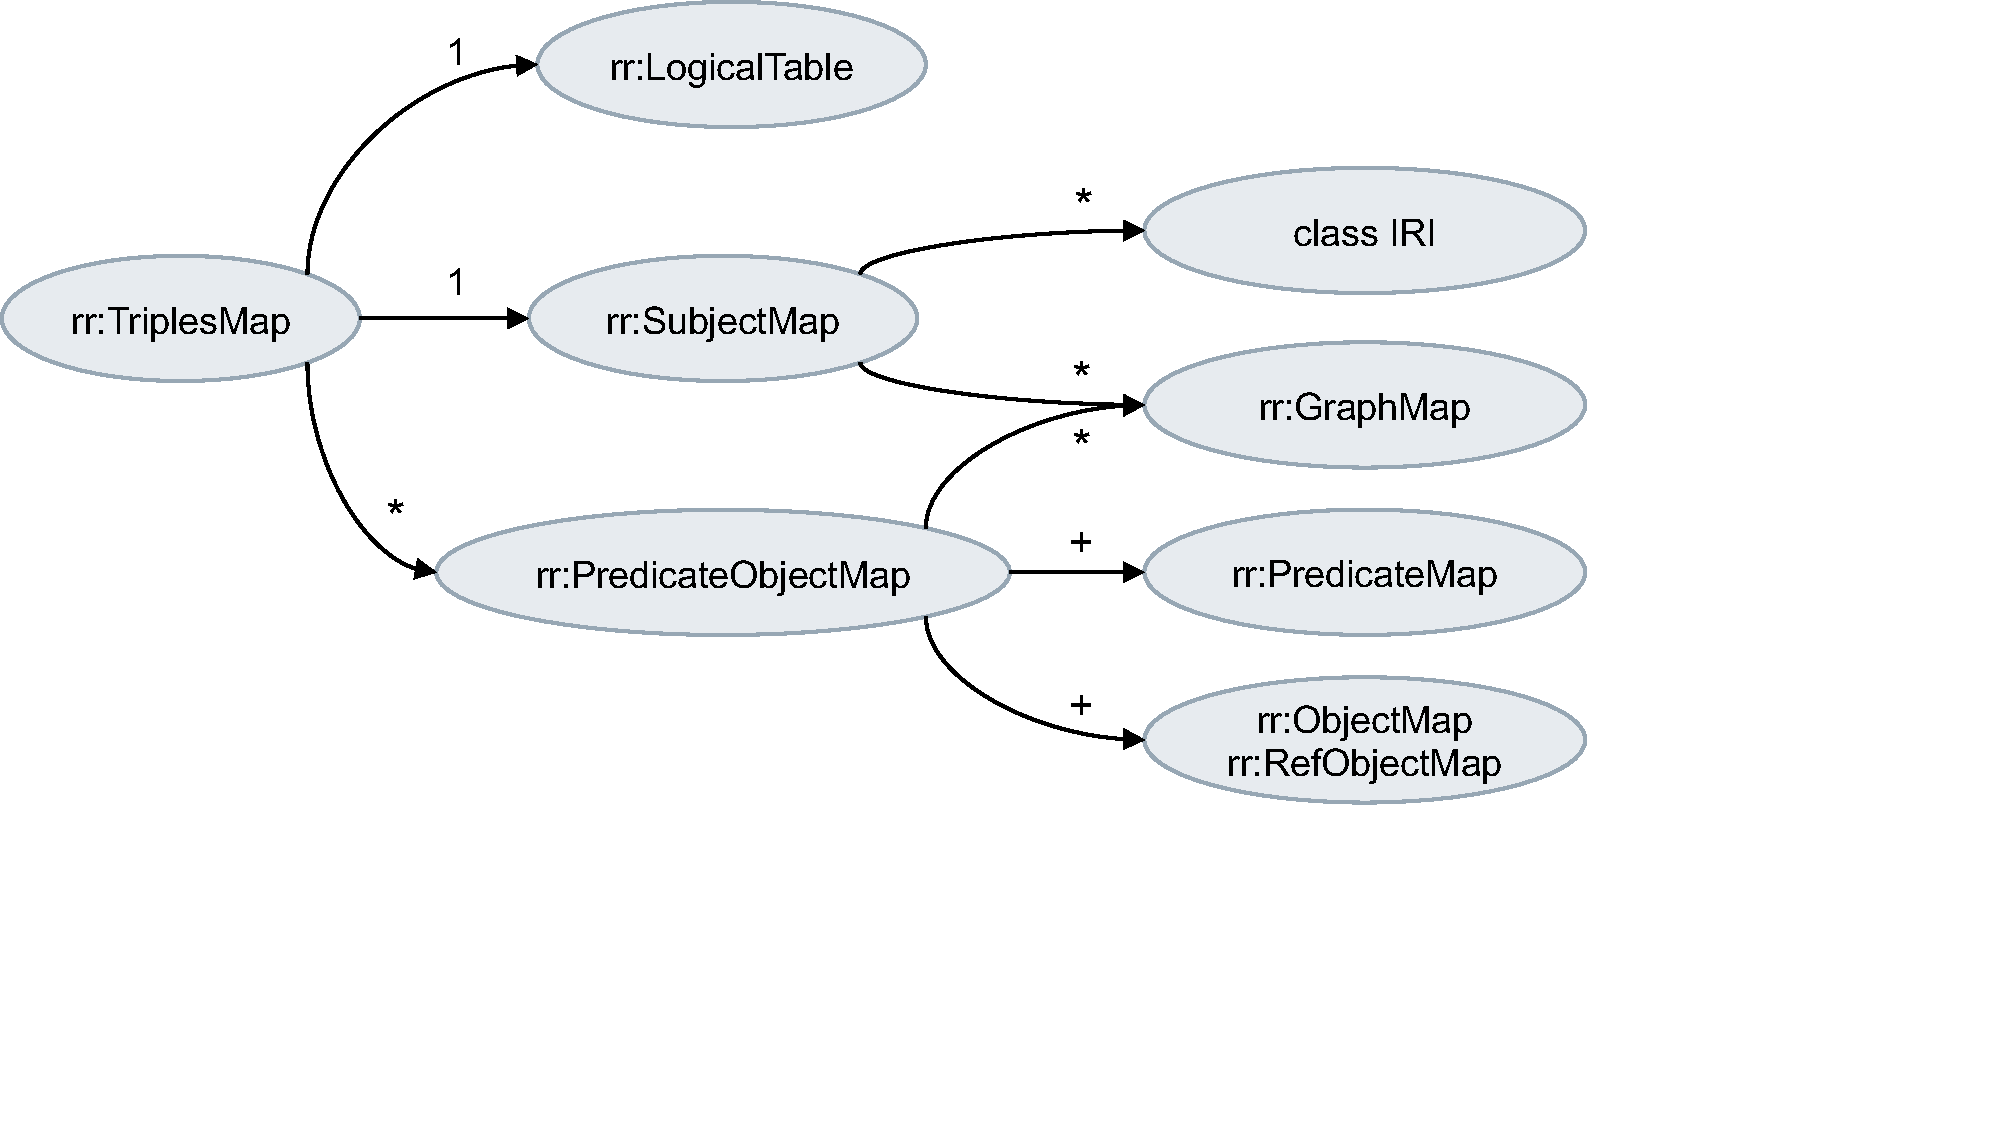
\includegraphics[width=0.7\linewidth]{figures/chp2_r2rml_tm.pdf}
\caption[Structure of Triples Map from R2RML]{Structure of a \textit{Triples Map} and its properties (adapted from \cite{das2012r2rml}).}
\label{fig:chp2_r2rml-tm}
\end{figure*}

\textit{Subject Map}, \textit{Predicate Map}, \textit{Object Map}, and \textit{Graph Map} are subclasses of \textit{Term Map} (\texttt{rr:TermMap}), which define how to generate RDF terms. 
\textit{Term Maps} can be (i) \textit{constant-valued} (\texttt{rr:constant}), i.e., always generating the same RDF term; 
(ii) \textit{column-valued} (\texttt{rr:column}), i.e., the RDF terms are directly obtained from cells of a column in the RDB; 
or (iii) \textit{template-valued} (\texttt{rr:template}), i.e., the RDF terms are composed from the data in columns and constant strings. These terms can be generated either as IRIs (\texttt{rr:IRI}), Blank Nodes (\texttt{rr:BlankNode}) or literals (\texttt{rr:Literal}) using \texttt{rr:termType}. The structure of a \textit{Term Map} is shown in \cref{fig:chp2_r2rml-term}.


\begin{figure*}[t]
\centering
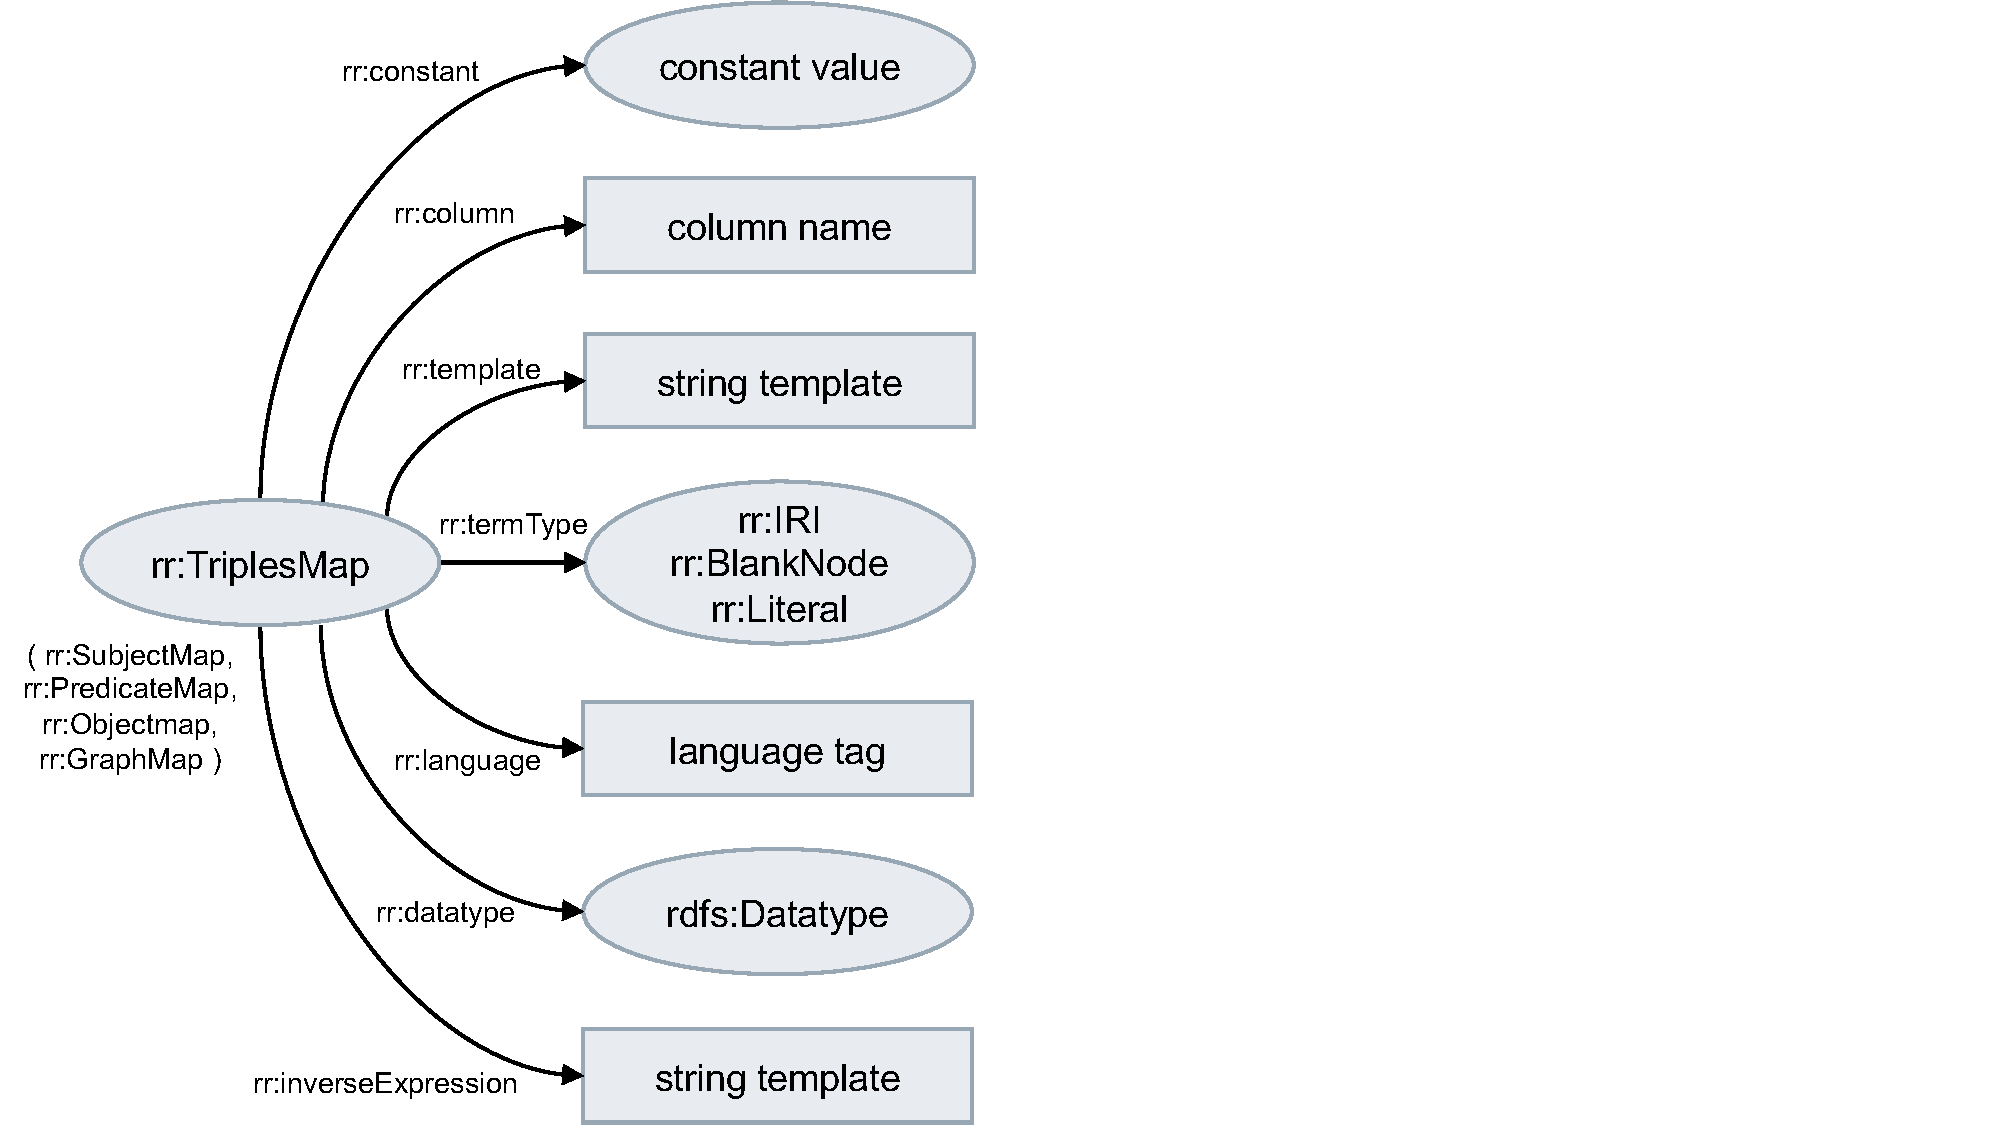
\includegraphics[width=0.45\linewidth]{figures/chp2_r2rml_term.pdf}
\caption[Structure of Triples Map from R2RML]{Structure of a \textit{Term Map} and its properties (adapted from \cite{das2012r2rml}).}
\label{fig:chp2_r2rml-term}
\end{figure*}



\cref{lst:chp2_r2rml-mapping} shows an example of an R2RML mapping to construct the RDF graph in \cref{lst:chp2_r2rml-result-rdf}. The R2RML mapping contains one \textit{Triples Map}, "TriplesMapAthletes" (Line 5). It takes as input the "Athletes" table shown in \cref{fig:chp2_database-example} (Line 6), which contains information about pole vault athletes, including their name, position in the ranking and height of a jump. The subject is formed with a template using one data source column (Line 8). The set of \textit{Predicate Object Maps} are used to describe with further attributes each instance (Lines 11-26). Two of them add the datatype to the object, one as an integer (Line 19) and other as a float (Line 25). 


\begin{figure*}[h]
\centering
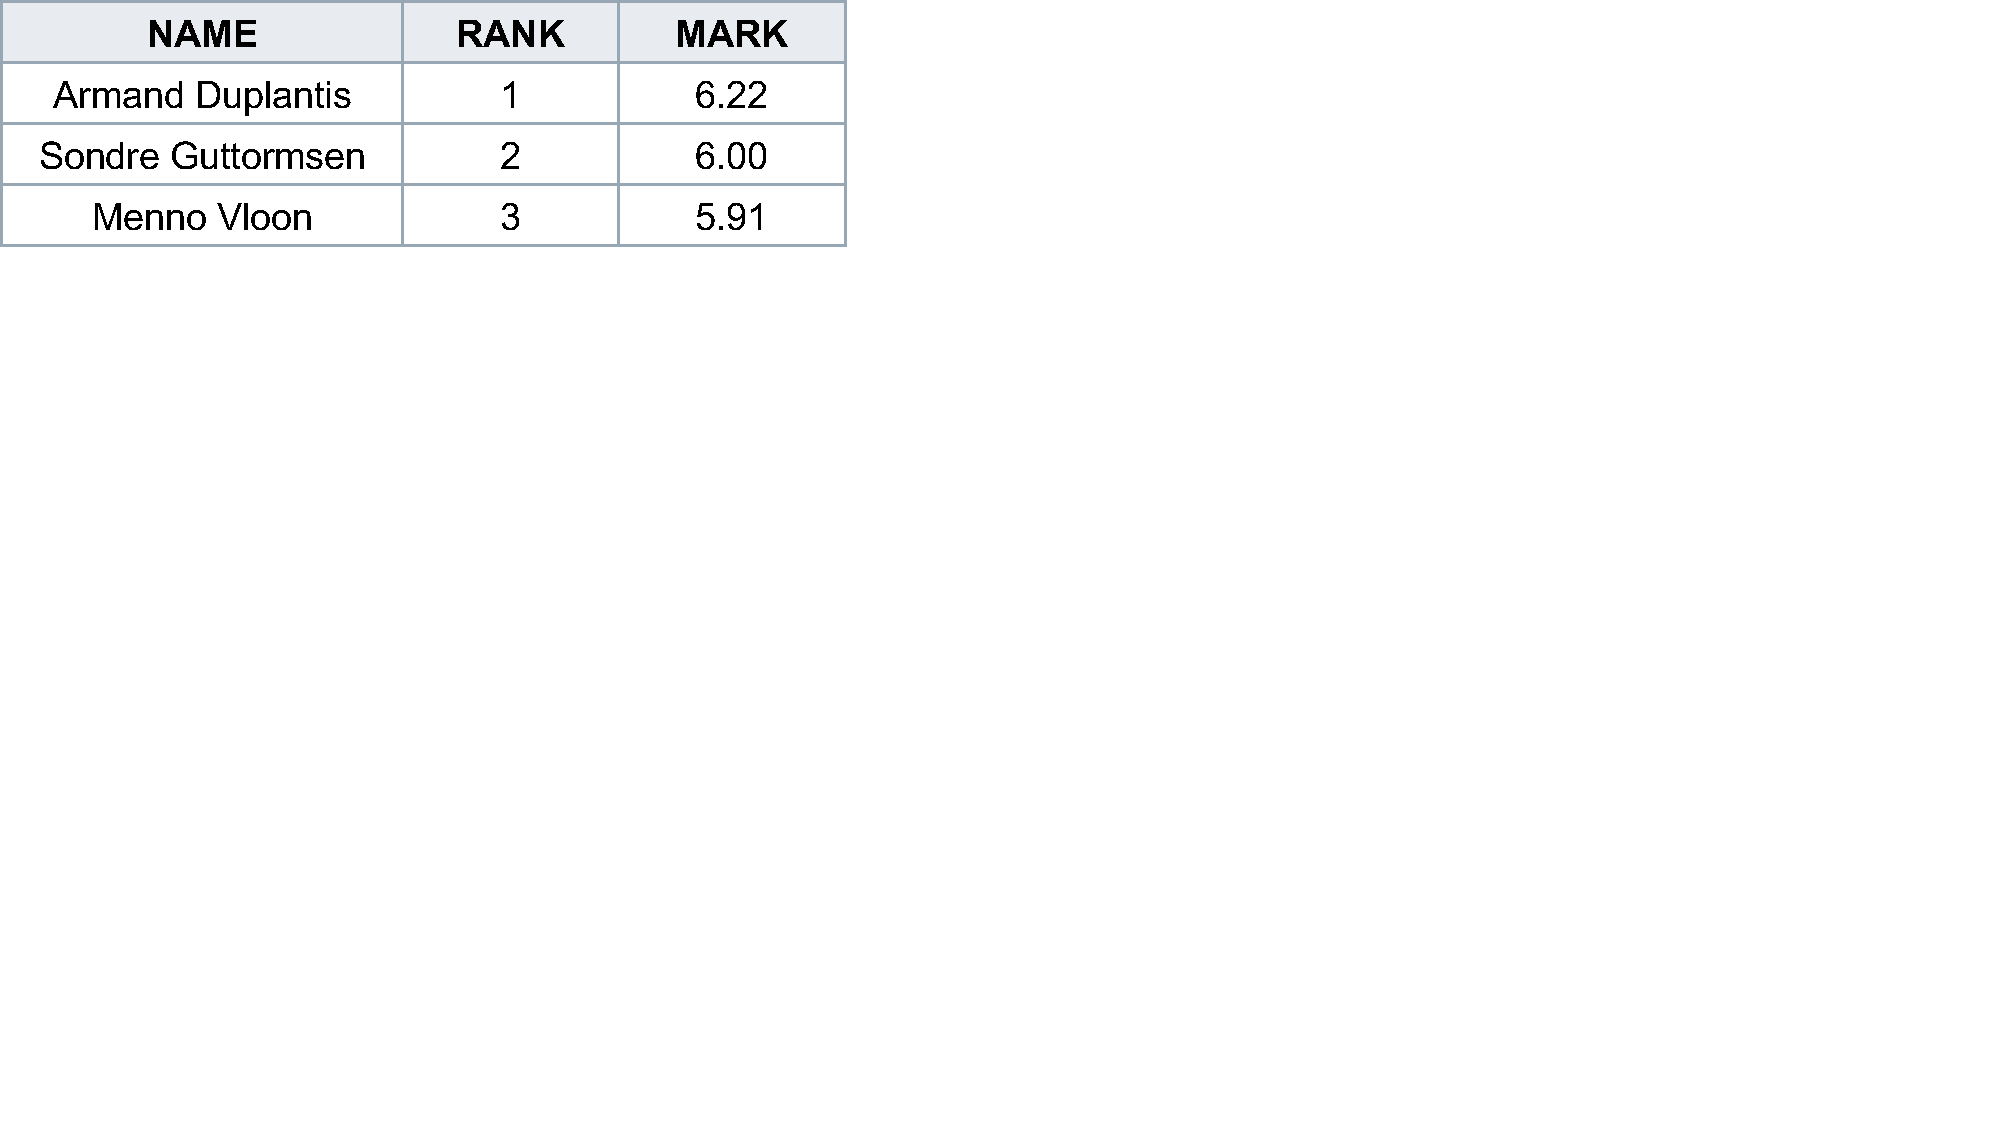
\includegraphics[width=0.45\linewidth]{figures/chp2_database-example.pdf}
\caption[Input "Athletes" table]{Input "Athletes" table with names, ranks and marks for athletes.}
\label{fig:chp2_database-example}
\end{figure*}

\begin{captionedlisting}{lst:chp2_r2rml-mapping}{R2RML mapping to generate the RDF graph in \cref{lst:chp2_r2rml-result-rdf} with data from the database table shown in \cref{fig:chp2_database-example}.}
\centering
{\begin{lstlisting}[language=r2rml]
@prefix rr: <http://www.w3.org/ns/r2rml#>.
@prefix xsd: <http://www.w3.org/2001/XMLSchema#>.
@prefix ex: <http://example.com/ns#>.

<#TriplesMapAthletes>
    rr:logicalTable [ rr:tableName "Athletes" ];
    rr:subjectMap [
        rr:template "http://example.com/athlete/{RANK}";
        rr:class ex:Athlete;
    ];
    rr:predicateObjectMap [
        rr:predicate ex:name;
        rr:objectMap [ rr:column "NAME" ];
    ];
    rr:predicateObjectMap [
        rr:predicate ex:rank;
        rr:objectMap [ rr:column "RANK" ; rr:datatype xsd:integer ];
    ];
    rr:predicateObjectMap [
        rr:predicate ex:mark;
        rr:objectMap [ rr:column "MARK" ; rr:datatype xsd:float ];
    ].
\end{lstlisting}}
\end{captionedlisting}

\begin{minipage}{\textwidth}
\begin{captionedlisting}{lst:chp2_r2rml-result-rdf}{RDF graph resulting from transforming data from the database table shown in \cref{fig:chp2_database-example} using the R2RML mapping in \cref{lst:chp2_r2rml-mapping}.}
\centering\begin{lstlisting}[language=r2rml]
ex:athlete/1 a ex:Athlete ;
    ex:name "Armand Duplantis" ;
    ex:rank "1"^^xsd:integer ;
    ex:mark "6.22"^^xsd:float .
ex:athlete/2 a ex:Athlete ;
    ex:name "Sondre Guttormsen" ;
    ex:rank "2"^^xsd:integer ;
    ex:mark "6.00"^^xsd:float .
ex:athlete/3 a ex:Athlete ;
    ex:name "Menno Vloon" ;
    ex:rank "3"^^xsd:integer ;
    ex:mark "5.91"^^xsd:float .
\end{lstlisting}
\end{captionedlisting}
\end{minipage}



 
\subsection{RML: RDF Mapping Language}
\label{sec:chp2_RML}
RML~\parencite{Dimou2014rml} extends R2RML to address the transformation of heterogeneous data formats, such as CSV, XML or JSON. It broadens the possibilities for KG construction with minimal changes in the vocabulary with respect to the standard. This language rapidly gained importance, and currently gathers an active community of users and developers. 

The main differences between RML and R2RML~\parencite{dimou2020rml-r2rml-diffs} are listed as follows:
\begin{itemize}
    \item \textbf{Data source reference}. RML introduces the \textit{Logical Source} (\texttt{rml:LogicalSource}), that extends R2RML's \textit{Logical Table}. The \textit{Logical Table} focuses on relational databases, whereas the \textit{Logical source} enables the description of more heterogeneous data sources in addition to relational databases.

    \item \textbf{Data source language}. In R2RML, the data source language is implicitly assumed to be SQL. To address heterogeneous data formats, RML uses the \textit{Reference Formulation} (\texttt{rml:ReferenceFormulation}) to indicate which formulation is suitable to parse data in a specific format. For instance, the JSONPath formulation can be used for parsing data in a JSON file. 

    \item \textbf{Iteration}. For tabular data sources, the iteration of the data source is per row. This strategy is followed by every R2RML processor to construct RDF graphs from RDBs. For non-tabular data sources, the iteration cannot always be implicitly assumed. For this reason, RML introduces the \textit{Iterator} (\texttt{rml:iterator})enabling the explicit determination of the iteration pattern to specify the specific data used in each iteration to build the RDF triples. The use of the \textit{Iterator} is optional, its use relies on the needs and particularities of each data source and use case.

    \item \textbf{Value reference}. R2RML relies on column names when referring to values in a table or view of a RDB (\texttt{rr:column}). RML broadens the scope of this concept using \textit{References} (\texttt{rml:reference}), that may refer to columns, objects (such as in the case of XML and JSON) or other elements valid with respect to the used \textit{Reference Formulation}. 
\end{itemize}


\cref{lst:chp2_rml-mapping} shows an example RML mapping that generates the same output RDF graph (\cref{lst:chp2_r2rml-result-rdf}) as the R2RML mapping previously shown in \cref{lst:chp2_r2rml-mapping}. Instead of a database table, this mapping takes as input a JSON file (\cref{lst:chp2_json-example}), which is described with the \textit{Logical Source)} (Lines 6-19). The fields of the input JSON file are referred to using the \texttt{rml:reference} property. 

\begin{minipage}{\textwidth}
\begin{captionedlisting}{lst:chp2_json-example}
{Input "Athletes.json" file with names, ranks and marks for athletes.}
\centering
\begin{lstlisting}[]
[ { "NAME": "Duplantis",
    "RANK": "1",
    "MARK": "6.22"},
  { "NAME": "Guttormsen",
    "RANK": "2",  
    "MARK": "6.00"},
  { "NAME": "Vloon",
    "RANK": "3",
    "MARK": "5.91"} ]
\end{lstlisting}
\end{captionedlisting}
\end{minipage}


\begin{captionedlisting}{lst:chp2_rml-mapping}{RML mapping to generate the RDF graph in \cref{lst:chp2_r2rml-result-rdf} with data from the JSON file shown in \cref{lst:chp2_json-example}.}
\centering
{\begin{lstlisting}[language=r2rml]
@prefix rr: <http://www.w3.org/ns/r2rml#>.
@prefix rml: <http://semweb.mmlab.be/ns/rml#>.
@prefix xsd: <http://www.w3.org/2001/XMLSchema#>.
@prefix ex: <http://example.com/ns#>.

<#TriplesMapAthletes>
  rml:logicalSource [
    rml:source "Athletes.json";
    rml:referenceFormulation ql:JSONPath;
    rml:iterator "$\dollar$.*"
  ];
    rr:subjectMap [
        rr:template "http://example.com/athlete/{RANK}";
        rr:class ex:Athlete;
    ];
    rr:predicateObjectMap [
        rr:predicate ex:name;
        rr:objectMap [ rml:reference "NAME" ];
    ];
    rr:predicateObjectMap [
        rr:predicate ex:rank;
        rr:objectMap [ rml:reference "RANK" ; rr:datatype xsd:integer ];
    ];
    rr:predicateObjectMap [
        rr:predicate ex:mark;
        rr:objectMap [ rml:reference "MARK" ; rr:datatype xsd:float ];
    ].
\end{lstlisting}}
\end{captionedlisting}

There are several proposals to extend the capabilities of RML. The initial features for addressing heterogeneous data sources were expanded by~\cite{Dimou2015Machine}, allowing more diverse data accesses and fine-grained description of the data sources. \cite{DeMeester2017fno_dbpedia} proposed \textbf{RML+FnO}, which provided RML with a connector to the Function Ontology~\parencite{demeester2016fno} to include data transformation functions in the mappings. \cite{delva2021rml-fields} introduced  \textbf{RML Fields}, that addressed several challenges to accurately access nested data. \textbf{RML Target} was developed by \cite{VanAssche2021LeveragingWebThings} to specify how to create the output triples regarding, for instance, RDF serialization, compression format or encoding. Lastly, \textbf{RML-star} was proposed by \cite{delva2021rml-star}, and later refined by \cite{arenas2023morphstar}, to allow the construction of RDF-star graphs. 

Recently, the Knowledge Graph Construction W3C Community Group\footnote{\url{https://www.w3.org/community/kg-construct/}} gathered these variety of specifications and released a new version of RML~\parencite{iglesias2023rml}, which includes several of these extensions, overcoming the identified limitations for declarative knowledge graph construction. This version is under standardisation.




\subsection{Additional Mapping Languages}
\label{sec:chp2_more-languages}

Following, we present an overview of existing mapping languages, listed in \cref{tab:chp2_languages_summary} and depicted in  \cref{fig:chp2_mapping_languages}. This section presents additional relevant languages classified in three categories, depending on the model they are based on or extend: (i)~RDF-based, (ii)~SPARQL-based, and (iii)~based on alternative schemas.


\begin{table}[t]
\caption[Mapping languages overview]{Analyzed mapping languages and their corresponding references.}
\label{tab:chp2_languages_summary}
\resizebox{\columnwidth}{!}{
\begin{tabular}{ccc}
%\rowcolor[HTML]{EFEFEF} 
\textbf{Classification}                 & \textbf{Language}        & \textbf{Reference(s)} \\ \midrule
\multirow{11}{*}{\textbf{RDF-based}}   & R2RML           & \parencite{das2012r2rml}\\ %\cmidrule{2-3} 
                              & RML             & \parencite{Dimou2014rml,rml}\\ %\cmidrule{2-3} 
                              & D2RQ            & \parencite{bizer2004d2rq,d2rq}\\ %\cmidrule{2-3} 
                              & XLWrap          & \parencite{langegger2009xlwrap,xlwrap}\\ %\cmidrule{2-3} 
                              & CSVW            & \parencite{Tennison2015csvw}\\ %\cmidrule{2-3}  
                              & KR2RML          & \parencite{slepicka2015kr2rml}\\ %\cmidrule{2-3} 
                              & xR2RML          & \parencite{michel2015xr2rml,xr2rml}\\ %\cmidrule{2-3} 
                              & R2RML-F         & \parencite{debruyne2016r2rmlf}\\ %\cmidrule{2-3} 
                              & FunUL           & \parencite{junior2016funul}\\ %\cmidrule{2-3} 
                              & R2RML for collections & \parencite{debruyne2017R2RML-collections}\\ %\cmidrule{2-3}   
                              & D2RML           & \parencite{chortaras2018d2rml}\\  \midrule
\multirow{5}{*}{\textbf{SPARQL-based}} & XSPARQL         & \parencite{Bischof2012xsparql,xsparql}\\ %\cmidrule{2-3} 
                              & TARQL           & \parencite{tarql}\\ %\cmidrule{2-3}
                              & SPARQL-Generate &     
                              \parencite{Lefrancois2017sparqlgenerate,sparqlgenerate}\\ %\cmidrule{2-3} 
                              & Facade-X        & \parencite{daga2021facade,sparqlanything}\\ %\cmidrule{2-3}
                              & NORSE            & \parencite{stadler2023spark}\\ \midrule
\multirow{4}{*}{\textbf{Alternative schema}}       & R$_2$O          & \parencite{barrasa2004r2o}\\ %\cmidrule{2-3}
                              & D-REPR          & \parencite{Vu2019d-repr}\\ %\cmidrule{2-3} 
                              & ShExML          & \parencite{Garcia-Gonzalez2020shexml,shexml}\\ %\cmidrule{2-3} 
                              & Helio mappings  & \parencite{cimmino2022helio}\\ 
                              \bottomrule
\end{tabular}}
\end{table}



\begin{figure*}[t]
\centering
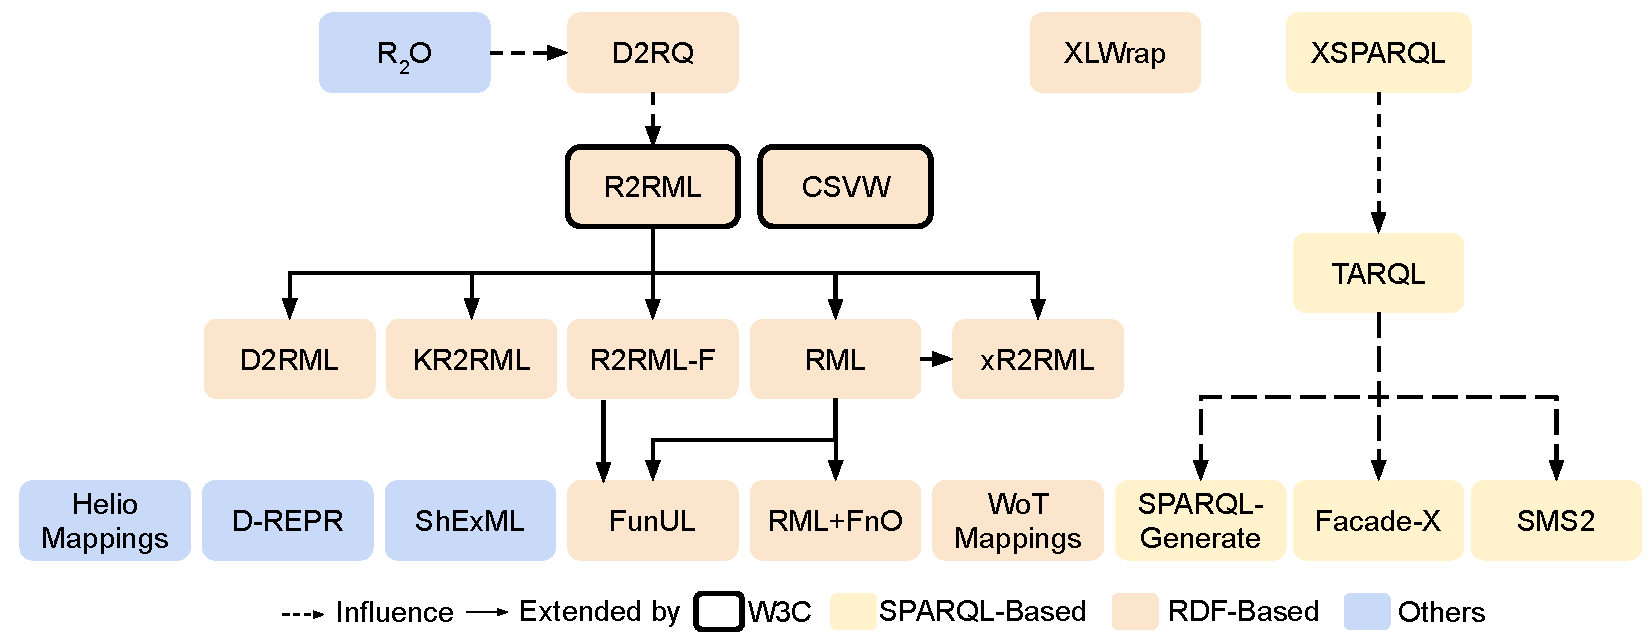
\includegraphics[width=1\linewidth]{figures/chp2_mapping_languages}
\caption[Existing mapping languages and the relationships among them]{Mapping languages developed in the last two decades, classified according to the schema they are based on, and the relationships among them.}
\label{fig:chp2_mapping_languages}
\end{figure*}




\subsubsection{RDF-based Mapping Languages.} 
\label{sec:chp2_RDF-languages}

Mapping languages in this group are formalized using RDF. They are usually modelled as ontologies or vocabularies that enable the description of data transformation rules. Mappings in these languages are usually written as files that follow the Turtle syntax~\parencite{turtle}. R2RML and RML, previously presented in \cref{sec:chp2_R2RML}
and \cref{sec:chp2_RML} respectively, also belong to this group of languages. 


\noindent\textbf{D2RQ}~\parencite{bizer2004d2rq} is one of the first mapping languages, developed to access the content of non RDF relational databases. The main components of this language are the \textit{Class Map} (\texttt{d2rq:ClassMap}) and the \textit{Property Bridge} (\texttt{d2rq:PropertyBridge})~\parencite{d2rq}. A \textit{Class Map} specifies how the instances of a class are generated, indicating the class that the instances belong to, the database's column(s) and URI pattern to create the URI for the instances. Each \textit{Class Map} also specifies the access to the input database, and refer to \textit{Property Bridges}. These \textit{Property Bridges} are used to generate the pairs of predicate-objects for the \textit{Class Map}, specifying the property for the predicate, and patterns and column references for the object. 


\noindent\textbf{XLWrap}~\parencite{langegger2009xlwrap} enables the transformation of spreadsheets to RDF. These mappings are written using the TriG syntax. They contain a graph instance of \texttt{xl:Mapping}, that describes the input file (workbook) (\texttt{xl:fileName}) and worksheet (\texttt{xl:sheetName}), a constant graph with information about the mapping (\texttt{xl:constantGraph}), references to \textit{Template Graphs} (\texttt{xl:templateGraph}) and \textit{Transformation Operations} (\texttt{xl:transformationOperation}). The \textit{Template Graphs} specify how to create the desired RDF graphs with references from the spreadsheet's cells and XLWrap expressions. This language provides further features to accurately access data in spreadsheets, described in the specification~\parencite{xlwrap}.  

\noindent\textbf{CSV on the Web (CSVW)}~\parencite{Tennison2015csvw} is a W3C Recommendation that enables a fine-grained annotation of CSV files and other tabular data formats, such as datatypes, valid values, data transformations, and primary and foreign key constraints. 

\noindent\textbf{KR2RML}~\parencite{slepicka2015kr2rml} extended R2RML to: (i) address multiple input data formats, such as CSV, JSON and XML; (ii) select the RDF serialization to create the output graph and (iii) integrate data transformation functions for pre-processing messy data without relying on SQL queries or views. To this end, the authors developed the nested Relational Model (NRM), as an intermediate form to represent data. NRM allowed the unification of the way to access data without loosing expressiveness. 

\noindent\textbf{xR2RML}~\parencite{michel2015xr2rml} extends R2RML and RML to include additional heterogeneous data sources and additional features not usually tackled by other mapping languages. It extends RML's \textit{Logical Source} to include NoSQL databases (e.g. MongoDB), and refines the access to different levels of iterations for hierarchical data sources with \texttt{xrr:pushDown}. It enables the creation of RDF lists and containers, by including additional \textit{Term Map} types (\texttt{xrr:RdfList}, \texttt{xrr:RdfSeq}, \texttt{xrr:RdfBag} and \texttt{xrr:RdfAlt}). Additionally, it allows the creation of dynamic language tags (i.e., with references from the input data) with \texttt{xrr:languageReference}.

\noindent\textbf{R2RML-F}~\parencite{debruyne2016r2rmlf} is a dedicated extension of R2RML to include data transformation functions, later refined in \textbf{FunUL}~\parencite{junior2016funul}. It introduces the \textit{Function} class (\texttt{rrf:Function}), which defines a data transformation function with name and body. An additional type of \textit{Term Map} is defined, the \textit{Function Valued Term Map}, which connects with the \textit{Function} and supplies it with parameter bindings. 

\noindent\textbf{R2RML for collections and containers}~\parencite{debruyne2017R2RML-collections} is another R2RML extensions focused on the generation of RDF lists and containers. These terms are created with \textit{Gather Maps}, that create a group of \textit{Object Maps} within an \textit{Object Map} with the \texttt{rrf:gather} property. 

\noindent\textbf{D2RML}~\parencite{chortaras2018d2rml} proposes a vocabulary extension to R2RML and RML with a large amount of features to describe in detail different heterogeneous data formats (e.g., JSON, CSV, XML) and accesses (e.g., RESTful APIs, SPARQL endpoints, documents) with a high level of detail. For instance, it adds to R2RML's \textit{Logical Table} and RML's \textit{Logical Source} the \textit{SQL Tables}, \textit{SPARQL Tables}, \textit{CSV Tables} and \textit{Information Source}. This proposal also includes data transformation functions to be used within the data source descriptions, and enables conditional generation of \textit{Term Maps}. 




\subsubsection{SPARQL-based Mapping Languages.}
\label{sec:chp2_SPARQL-languages} 

This group is integrated by languages that leverage the SPARQL query language, usually by extending its features to describe non-RDF data sources~\parencite{harris2013sparql}. 


\noindent\textbf{XSPARQL}~\parencite{Bischof2012xsparql} combines XQuery and SPARQL to enable the transformation between XML and RDF data sources bidirectionally. This language inherits all inherent features of both languages, excluding the \texttt{ASK} and \texttt{DESCRIBE} query forms. To perform the translation from XML to RDF, the data is extracted using the XQuery language with variables, that are later used in a \texttt{CONSTRUCT} clause to create the RDF graph. 

\noindent\textbf{TARQL}~\parencite{tarql} allows CSV transformation using the SPARQL syntax. The columns names of the input CSV files are treated as variables, which can be used in a \texttt{CONSTRUCT} clause to construct the RDF graph. The input file is referred to using the \texttt{FROM} clause. 

\noindent\textbf{SPARQL-Generate}~\parencite{Lefrancois2017sparqlgenerate} presents a more holistic approach than its predecessors providing access to more than one input data source format. This language is capable of generating RDF and text streams from a wide variety of data formats and access protocols. To this end, it introduces three new clauses to the SPARQL syntax: (i) \texttt{SOURCE} to bind variables to the input data source, (ii) \texttt{ITERATOR} to for accurately extracting data from the data sources; and (iii) \texttt{GENERATE}, that replaces and extends the \texttt{CONSTRUCT} clause with embedded SPARQL-Generate queries. 

\noindent\textbf{Facade-X}~\parencite{daga2021facade} is proposed to also deal with a variety heterogeneous data sources relying in the SPARQL syntax, but without extending it with additional clauses. This proposal overrides the \texttt{SERVICE} operator to access heterogeneous data that can be queried as if it was RDF with a \textit{façade}. Hence, data is retrieved in the \texttt{SERVICE} operator and bound as variables, that are later used in the \texttt{CONSTRUCT} clause to construct RDF graphs. 

\noindent\textbf{NORSE}~\parencite{stadler2023spark} was developed as a vocabulary to place non-RDF data source descriptions within the SERVICE operator. This vocabulary allows including RML \textit{Logical Source} descriptions inside queries, bound to SPARQL variables. In this approach, graphs are also generated using the \texttt{CONSTRUCT} clause. 




%\textit{XSPARQL~\parencite{Bischof2012xsparql} merges SPARQL and XQuery to transform XML into RDF. TARQL~\parencite{tarql} uses the SPARQL syntax to generate RDF from CSV files. SPARQL-Generate~\parencite{Lefrancois2017sparqlgenerate} is capable of generating RDF and document streams from a wide variety of data formats and access protocols. Most recently, Facade-X has been developed, not as a new language, but as a "\textit{facade} to wrap the original resource and to make it queryable as if it was RDF"~\parencite{asprino2023sparql-anything}. It does not extend the SPARQL language, instead it overrides the SERVICE operator. Lastly, authors would like to highlight a loosely SPARQL-based language, Stardog Mapping Syntax 2 (SMS2)~\parencite{sms2}, which represents virtual Stardog graphs and is able to support sources such as JSON, CSV, RDB, MongoDB and Elasticsearch.}




\subsubsection{Mapping Languages Based on Alternative Schemas.} 
\label{sec:chp2_alternative-languages}

Lastly, the languages of this group rely on models different from RDF or SPARQL, equally able and expressive enough to allow users to write transformation rules. 


\noindent\textbf{R$_2$O}~\parencite{barrasa2004r2o} is an XML-based language able to describe the transformation rules for constructing graphs from relational databases. %Its vocabulary relies on three main concepts: \textit{Concept Maps}, \textit{Attribute Maps} and \textit{Relation Maps}. 
An R$_2$O mapping consists on the following components: description of the database schema, ontology URI(s), mapping definitions between the ontology and database, and optionally a set of instance URIs to be added. The mapping definitions enable the description on how to generate the triples, as well as conditional expression, joins over the data source elements and data transformation functions. 

%~\footnote{https://pdfs.semanticscholar.org/4c47/0826aafc07fc6d37ca7e2474c1d3b290ade1.pdf}

\noindent\textbf{D-REPR}~\parencite{Vu2019d-repr}, Dataset REPResentation language, can be written as YAML or JSON files, providing a user-friendly approach to describe the transformation rules from a wide range of data source formats. This language requires four components: dataset resources, attributes of data sources, a semantic model to map the attributes to the ontology classes, and rules for the values of the attributes. This language also enables the use of data transformation functions. 

\noindent\textbf{ShExML}~\parencite{Garcia-Gonzalez2020shexml,shexml} proposes a mapping language based on the ShEx validation language for knowledge graphs~\parencite{prud2014shex}. This language enables the access to heterogeneous data sources, such as JSON, XML, CSV, RDBs and RDF with SPARQL queries. A ShExML mapping is divided in a declaration and a generation part. The declaration part provides the specification of prefixes, data sources, iterators, fields and expressions for merging or transforming data. The generation part describes how to generate triples and graphs with the fields and expressions defined in the declaration part. 

\noindent\textbf{Helio}~\parencite{cimmino2022helio} is a JSON-based language that provides a variety of possibilities for heterogeneous data formats and accesses, as well as for extended functions for linking resources further than left joins, and data transformation functions. A Helio mapping is composed of a \textit{data source} description, defining also its provider and handler; a set of \textit{resource rules} that conform the triple generation rules; and optionally a set of \textit{linking rules} to be applied over the resource rules. 








\subsection{Mapping Languages Expressiveness Comparison}
\label{sec:chp2_language-comparison}

As the number of mapping languages increased and their adoption for KG construction grew wider, comparisons among these languages started emerging. This is the case of, for instance, SPARQL-Generate~\parencite{Lefrancois2017sparqlgenerate}, which is compared to RML in terms of query/mapping complexity; and ShExML~\parencite{Garcia-Gonzalez2020shexml}, which is compared to SPARQL-Generate and YARRRML from a usability perspective.

Some studies dig deeper, providing qualitative complex comparison frameworks. \cite{hert2011comparison} provide a comparison framework for mapping languages focused on transforming relational databases to RDF. The framework is composed of 15 features: Logical table to class, M:N relationships, project attributes, select conditions, user-defined instance URIs, literal to URIs, vocabulary reuse, transformation functions, datatypes, named graphs, blank nodes, integrity constraints, static metadata, one table to \textit{n} classes, and write support. 
The results lead authors to divide the mappings into four categories (direct mapping, read-only general-purpose mapping, read-write general-purpose mapping, and special-purpose mapping), and ponder on the heavy reliance of most languages on SQL to implement the mapping, and the usefulness of read-write mappings (i.e., mappings able to write data in the database). \cite{DeMeester2019comparison} show an initial analysis of 5 similar languages (RML+FnO, xR2RML, FunUL, SPARQL-Generate, YARRRML) discussing their characteristics, according to three categories: non-functional, functional and data source support. The study concludes by remarking on the need to build a more complete and precise comparative framework and asking for a more active participation from the community to build it. 

More recently, two related systematic reviews were published. \cite{vanassche2023survey} focused specifically on declarative KG construction. This survey analyses the characteristics of mapping languages assessing 15 characteristics for schema transformations and 5 for data transformation; as well as of compliant systems with 14 characteristics. It provides a more in-depth and systematic analysis than previous studies, but it is limited to reviewing peer-reviewed publications. Then, the expressiveness of languages such as R2RML, CSVW or TARQL that lack this kind of publication are not included. The review presented by \cite{ryen2022kgreview} was more limited in extension with respect to \cite{vanassche2023survey}, but broader in scope considering knowledge graph generation and publication. %Finally, \cite{tamavsauskaite2023defining} defines a common set of steps for developing knowledge graphs, based on the processes followed for building and deploying existing knowledge graphs. 

\ana{add takeaway}

\subsection{Interoperability for Mapping Languages}
\label{sec:chp2_interoperability}

The large amount of mapping languages presented in this section opens the door to a wide range of possibilities for KG construction. The downside of this situation comes with the general lack of interoperability among them~\parencite{corcho2020towards}. Each mapping processor usually provides support for one mapping language, therefore, forcing users to learn different languages depending on the features that the language and compliant engine can provide to tackle the needs of each use case. 

We find some examples of unidirectional pairwise translations between these languages. 
Helio and SPARQL-Generate, with the aim of extending their outreach, implement a plugin to translate from RML to their corresponding compliant language\footnote{\url{https://github.com/oeg-upm/helio/wiki/Streamlined-use-cases\#materialising-rdf-from-csv--xml-and-json-files-using-rml}}$^,$\footnote{\url{https://helio-playground.linkeddata.es/tour}}$^,$\footnote{\url{https://github.com/sparql-generate/rml-to-sparql-generate}}. Inversely, ShExML provides translation to RML in its playground\footnote{\url{https://shexml.herminiogarcia.com/editor/}}, thus presenting the language also as a user-friendly syntax for RML~\parencite{Garcia-Gonzalez2020shexml}. 

There are also examples of tools that provide a set of optimizations for KG construction exploiting the translation of mapping rules. This is the case of Morph-CSV~\parencite{chaves2021morph-csv} and FunMap~\parencite{jozashoori2020funmap}. Morph-CSV performs a transformation over the tabular data with RML+FnO mappings and CSVW annotations, and outputs a database and R2RML mappings. FunMap takes an RML+FnO mapping, performs the transformation functions indicated, outputs the parsed data and generates a function-free RML mapping.

Lastly, the user-friendly serializations presented later in the chapter are always supported with translations to a mapping language, which is explained in detail in \cref{sec:chp2_easy_kgc}.


\ana{add takeaway}

%Another case is when tools implement RML/R2RML mapping translation into the language they are designed to parse; such as Helio\footnote{\url{https://github.com/oeg-upm/helio/wiki/Streamlined-use-cases\#materialising-rdf-from-csv--xml-and-json-files-using-rml}} and SPARQL-Generate\footnote{\url{https://github.com/sparql-generate/rml-to-sparql-generate}}, that translate from RML to their respective language; and Ontop~\cite{calvanese2017ontop}, that translates R2RML into its compliant language

\section{User-Friendly Knowledge Graph Construction Approaches}
\label{sec:chp2_easy_kgc}

\ana{dividir o serializations/editores, o manual/semi/automatic o algo así}

\section{Knowledge Graph Lifecycle \textcolor{red}{-- By 2/2}}
\label{sec:chp2_kg_lifecycle}

\ana{repasar un poco los papers que hablen de ciclo de vida de KGs, dónde encajan los mappings ahí y qué se ha estudiado en su intervención en el proceso, para decir que en la evolución no se ha estudiado}

\section{Conclusions and Limitations of the State of the Art}
\label{sec:chp2_conclusions-sota}

This chapter presents the relevant work in the state of the art about declarative mapping languages for knowledge graph construction and evolution. 
We conclude in this section with the identification of the challenges in the field that motivate the contributions of this thesis, which are presented in the following chapters.

\begin{itemize}
    \item \textbf{Different mapping language expressiveness and processing characteristics of their associated engines.} Many different mapping languages for knowledge graph construction from heterogeneous data sources have been released over the years. These languages offer a differential set of features, providing a wide variety of possibilities for addressing real-world use cases. Deciding which language is the most suitable for the particularities of each use case and requirements becomes hard without a fine-grained comparison of the features that each language provides. 
    
    \item \textbf{Updating mapping languages according to new needs.} As KG technologies advance, new needs and requirements emerge in KGC. Despite the options that mapping languages currently provide, they have limitations and have not adopted yet some of the latest developments (e.g. the currently work in progress RDF 1.2 specification~\parencite{hartig2023rdf}). These limitations negatively impact on the adoption of declarative approaches for KGC, as they must be competitive with ad-hoc approaches (e.g. programming scripts) in terms of expressiveness and keep up with the current progress in the field.
    
    \item \textbf{Adoption barrier for writing declarative mappings.} Mappings usually follow a syntax that is not easy or intuitive to write, especially for non-experts. Several developments have been released, providing user interfaces and user-friendly serializations to improve the writing task for users. However, visual approaches have not been adopted in general, and serializations still pose a barrier for users with non-technical profiles. 

    %\item \ana{interoperability issue? not a contribution (in chp3) for now}
    
    \item \textbf{The role of declarative mappings in the knowledge graph life cycle.} Mapping languages were developed for constructing KGs from diverse data sources, relating them to the schema provided by an ontology. However, the analysis show that they can also be part of other tasks of the KG life cycle, such as data pre-processing and metadata annotation. Yet, the role that they can play in other parts of the life cycle has not been assessed. 
\end{itemize}
